\usetikzlibrary{matrix}
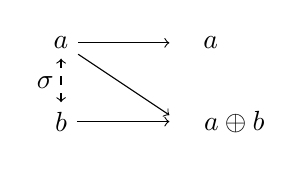
\begin{tikzpicture}
\node (a) at (0,0) {$a$};
\node (b) at (0,-1) {$b$};

\node (a2) at (1.5,0) {};
\node (ab) at (1.5,-1) {$$};

\node at (1.9,0) {$a$};
\node at (2.2,-1) {$a \oplus b$};

\node at (-0.2, -0.5) {$\sigma$};

\draw[->] (a)--(a2);
\draw[->] (a)--(ab);
\draw[->] (b)--(ab);

\draw[<->, dashed] (a)--(b);

\end{tikzpicture}